%%%%%%%%%%%%%%%%%%%%%%%%%%%%%%%%%%%%%%%%%
% Beamer Presentation
% LaTeX Template
% Version 1.0 (10/11/12)
%
% This template has been downloaded from:
% http://www.LaTeXTemplates.com
%
% License:
% CC BY-NC-SA 3.0 (http://creativecommons.org/licenses/by-nc-sa/3.0/)
%
%%%%%%%%%%%%%%%%%%%%%%%%%%%%%%%%%%%%%%%%%

%----------------------------------------------------------------------------------------
%	PACKAGES AND THEMES
%----------------------------------------------------------------------------------------

\documentclass{beamer}

\mode<presentation> {

% The Beamer class comes with a number of default slide themes
% which change the colors and layouts of slides. Below this is a list
% of all the themes, uncomment each in turn to see what they look like.

%\usetheme{default}
%\usetheme{AnnArbor}
%\usetheme{Antibes}
%\usetheme{Bergen}
%\usetheme{Berkeley}
%\usetheme{Berlin}
%\usetheme{Boadilla}
%\usetheme{CambridgeUS}
%\usetheme{Copenhagen}
%\usetheme{Darmstadt}
%\usetheme{Dresden}
%\usetheme{Frankfurt}
%\usetheme{Goettingen}
%\usetheme{Hannover}
%\usetheme{Ilmenau}
%\usetheme{JuanLesPins}
%\usetheme{Luebeck}
\usetheme{Madrid}
%\usetheme{Malmoe}
%\usetheme{Marburg}
%\usetheme{Montpellier}
%\usetheme{PaloAlto}
%\usetheme{Pittsburgh}
%\usetheme{Rochester}
%\usetheme{Singapore}
%\usetheme{Szeged}
%\usetheme{Warsaw}

% As well as themes, the Beamer class has a number of color themes
% for any slide theme. Uncomment each of these in turn to see how it
% changes the colors of your current slide theme.

%\usecolortheme{albatross}
%\usecolortheme{beaver}
%\usecolortheme{beetle}
%\usecolortheme{crane}
%\usecolortheme{dolphin}
%\usecolortheme{dove}
%\usecolortheme{fly}
%\usecolortheme{lily}
%\usecolortheme{orchid}
%\usecolortheme{rose}
%\usecolortheme{seagull}
%\usecolortheme{seahorse}
%\usecolortheme{whale}
%\usecolortheme{wolverine}

%\setbeamertemplate{footline} % To remove the footer line in all slides uncomment this line
%\setbeamertemplate{footline}[page number] % To replace the footer line in all slides with a simple slide count uncomment this line

%\setbeamertemplate{navigation symbols}{} % To remove the navigation symbols from the bottom of all slides uncomment this line
}

\usepackage{graphicx} % Allows including images
\usepackage{booktabs} % Allows the use of \toprule, \midrule and \bottomrule in tables
\usepackage[czech]{babel}
%----------------------------------------------------------------------------------------
%	TITLE PAGE
%----------------------------------------------------------------------------------------

\title[amogus]{Základy počítače} % The short title appears at the bottom of every slide, the full title is only on the title page

\author{Jáchym Löwenhöffer} % Your name
\institute[GEVO] % Your institution as it will appear on the bottom of every slide, may be shorthand to save space
{
Gynekologická Evaluace Velkých Obrazů \\ % Your institution for the title page
\medskip
\textit{jachym.lowenhoffer@gmail.com} % Your email address
}
\date{\today} % Date, can be changed to a custom date



\AtBeginSection[]
{
  \begin{frame}
  \vfill
  \centering
  \begin{beamercolorbox}[sep=8pt,center,shadow=true,rounded=true]{title}
    \usebeamerfont{title}\insertsectionhead\par%
  \end{beamercolorbox}
  \vfill
  \end{frame}
}

\begin{document}

\begin{frame}
	\titlepage % Print the title page as the first slide
\end{frame}

\begin{frame}
	\frametitle{Přehled} % Table of contents slide, comment this block out to remove it
	\tableofcontents % Throughout your presentation, if you choose to use \section{} and \subsection{} commands, these will automatically be printed on this slide as an overview of your presentation
\end{frame}

%----------------------------------------------------------------------------------------
%	PRESENTATION SLIDES
%----------------------------------------------------------------------------------------

%------------------------------------------------
\section{Co je v počítači} % Sections can be created in order to organize your presentation into discrete blocks, all sections and subsections are automatically printed in the table of contents as an overview of the talk
%------------------------------------------------



\begin{frame}
	\frametitle{Paměť a registry}
	%------------------------------------------------
	\begin{itemize}
		\item \textbf{Paměť} je na sobě naházená jako na hromadě, ale každý byte má svojí
		      adresu.
		\item  \textbf{Registr} je chlíveček, kam schovám byte a můžu s ním pracovat
		      (porovnávat, sčítat atd.).
		\item \textbf{Address Bus}: tudy se posílají adresy.
		\item \textbf{Data Bus}: tudy se posílají data.
		\item \textbf{PC}(program counter): je speciální registr kam se ukládá adresa další instrukce
		 na vykonání.
		\item \textbf{MBR}: je část paměti kam se uloží
		 instrukce na vykonání předtím než se posune do místa kde se opravdu může
		 vykonat.
	\end{itemize}
\end{frame}

\section{FDE cycle}
\label{sec:fde-cycle}

\begin{frame}
 \frametitle{Fakt Drsná Elipsa}
 \includegraphics[scale=0.25]{elipsa.jpg}
\end{frame}

\begin{frame}
\frametitle{Program? jako co budou večer dávat?}

\begin{block}{Počítačový program}
je posloupnost instrukcí, která má nějaký cíl. Může mít nějaký vstup, ale výstup
mít musí!
\end{block}

Jestliže budeme mít program který hledá třetí mocninu čísel tak mu ale musíme
dát nějaké číslo aby nám mohl něco vrátit. Toto číslo je tedy vstup. Výstupem je
výsledek nebo eror.
\end{frame}



\begin{frame}
	\frametitle{\textbf{F}etch [vyzvedni]}
	\begin{itemize}
		\item CPU se podívá na svůj PC (program counter), tam je uložena adresa další
		      instrukce.
		\item Address busem pošle pro tuto instrukci do RAMky (tam už musí být
		 předem celý program načtený)
		\item Data busem se vrátí hodnota této instrukce.
		\item Zapíše se do MBR a z něj se zkopíruje do CIR (current instruction
		      register).
		     \item CIR je registr, kde je CPU schopná instrukci vykonat a tím
		     	zaúkolovat další registry.
	\end{itemize}
\end{frame}


\begin{frame}
	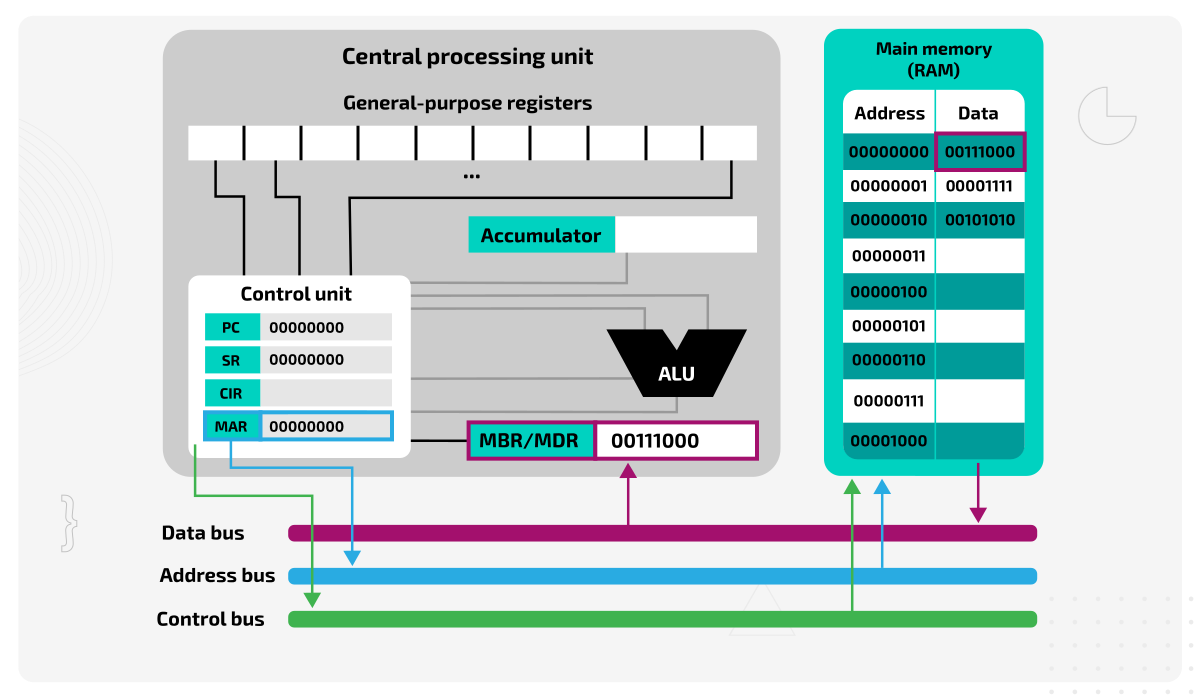
\includegraphics[scale=0.3]{fde.png}
\end{frame}

%------------------------------------------------

\begin{frame}
	\frametitle{\textbf{D}ecode}

	\begin{itemize}
		\item Jakmile je instrukce v CIR (, CPU začne hledat, o jakou instrukci jde.
		\item To udělá tak, že ji rozdělí na části.
		\item Podle typu instrukce vyvěsí \emph{vlajky}\footnote{Programu říkají, že se
			      děje něco zajímavého a on na ně může reagovat.} nebo připraví potřebné registry.
		\item Taky se hodnota v PC zvýší o jedna, aby se tím program posunul na
		      další instrukci.
	\end{itemize}
\end{frame}


\begin{frame}
	\frametitle{\textbf{E}xecute}
	\begin{itemize}
		\item Jakmile víme o jakou instrukci se jedná, můžeme ji vyhodnotit!
		\item Jaké instrukce existují?
	\end{itemize}
\end{frame}

\section{Instrukce}
\label{sec:instrukce}

\begin{frame}
	\frametitle{Řídící}
	\begin{description}
		\item[\texttt{jump}] přepíše hodnotu v PC (adresa další instrukce na vykonání)
		      na nějakou jinou. Díky tomu můžeme mít věci jako \emph{cykly}.
		\item[\texttt{jump-if}] to samé jako \texttt{jump}, jen předtím ověří nějakou
		      podmínku. Porovná hodnoty dvou registrů nebo ověří nějaké
		      \emph{vlajky}. Tedy se tato instrukce nápadně podobá \emph{podmínkám}
		      v programování.
	\end{description}
	
	Oba skoky můžou být na jakékoliv místo v paměti a náš program tak vůbec nemusí být
	pohromadě tak jak jsme ho napsali. Což vůbec nevadí a jediné co nás zajímá je
	aby byl proveden v takovém pořadí.
\end{frame}


\begin{frame}
	\frametitle{Paměťové}
	\begin{description}
		\item[\texttt{alocate}] vyhradí pro náš program kus prostoru v paměti a
		      všechny ostatní programy vědí, že tuto část nemají používat. Jakmile už ji
		      nepotřebujeme, je třeba tuto paměť uvolnit.
		\item[\texttt{load}] načte určitý úsek z paměti do registrů.

		\item [\texttt{store}] hodnoty z registrů (třeba výsledek výpočtu)
		      uloží do paměti.
	\end{description}
\end{frame}
%------------------------------------------------

\begin{frame}
	\frametitle{Výpočetní}
	\begin{description}
		\item[\texttt{add}] sečte hodnotu ze dvou registrů a uloží ji do třetího.
		\item[\texttt{compare}] porovná hodnoty ve dvou registrech a výsledek uloží do
		      třetího. Výsledek je vždy \texttt{true} nebo \texttt{false}.
	\end{description}
\end{frame}

\section{Logické obvody}
\label{sec:logicke-obvody}

\begin{frame}
	\frametitle{Od logiky k počítači}
	Kdybychom měli jen dráty uchovávající jedničky a nuly, tak je nuda. Potřebujeme
	ještě způsob, jak mezi sebou tyto signály kombinovat, potřebujeme na nich
	nějakou logiku.

	\vfill

	Proto máme logické brány. Pomocí těchto bran jsme schopni postavit celé moderní
	počítače.

	\vfill

	\begin{block}{Logická brána}
	 Je jednoduchý obvod, který vezme nějaký počet drátů a jejich napětí jako
	 vstup a vydá výstup, který je závislý na vstupu.
	\end{block}
\end{frame}

\begin{frame}
	\frametitle{Logické brány}
	\begin{description}
		\item[\texttt{AND}] funguje stejně jako v jazyce. Výrok: "Venku je zima a
		 prší." je pravdivý, jen když venku opravdu prší a opravdu je zima.
		\item[\texttt{OR}] také se dá najít v jazyce. Funguje jako "nebo" ve
		      slučovacím poměru.
		\item[\texttt{NOT}] otáčí původní hodnotu signálu. Jestliže je vstup 0, tak
		      vrátí 1, a naopak.
	\end{description}

	Než nám to nadcházející obrázek prozradí zamysleme se, nad tím jak bychom
	logické brány reprezentovali jako aritmetické operace v binární soustavě.
\end{frame}

\begin{frame}
	\frametitle{Tabulky pravdivostních hodnot}
	\includegraphics[scale=0.14]{gates.jpg}
\end{frame}

\begin{frame}
\frametitle{\texttt{NA(n)D}e vše!}
 Logických brán je samozřejmě o hodně víc než jen tyto tři. Kdybyste si někdy
 chtěli stavět vlastní procesor hodí se vědět, že jich tolik vlastně
 nepotřebujete. Úplně vám stačí brána \texttt{AND} a \texttt{NOT}. Ty když dáme
 hned za sebe (ve stejném pořadí) vznikne nám \texttt{NAND}.

 \includegraphics[scale=0.35]{nand.png}
\end{frame}

\begin{frame}
 \frametitle{Výlučné \texttt{OR}}
 Aby toho nebylo málo ukážeme si ještě jako udělat výlučné \texttt{OR}, tedy
 \texttt{XOR}. Jedná se o \texttt{OR} jen s tou vyjímkou, že když jsou oba
 vstupy pravda výstupem je nepravda. Ptáme se tedy na otázku: \uv{Je
 	\textbf{právě jeden}
 vstup pravda?} namísto \uv{Je \textbf{alespoň} jeden vstup pravda?} jak je
 tomu u \texttt{OR}.

 \includegraphics[width=\textwidth]{xor.png}
\end{frame}


\begin{frame}
	\frametitle{Jednoduchý logický obvod}
	\includegraphics[width=\textwidth]{circut-0000.jpg}
\end{frame}

\begin{frame}{Konečně sčítáme!}
 \includegraphics[scale=0.9]{Screenshot from 2024-09-19 11-10-26.png}
\end{frame}


\section{Paměť}
\label{sec:pamet}

\begin{frame}
	\frametitle{Volatilní vs. nevolatilní}
	\begin{block}{Volatilita}
		je nutnost paměti být připojena na stálé napětí. Jakmile ho jednou odpojíme,
		ztrácíme všechna data.
	\end{block}
	U té nevolatilní ztrácíme jen možnost z ní číst a do ní psát, což je přirozené.
\end{frame}

\begin{frame}
	\frametitle{Proč RAM?}
	RAMka je nejrozšířenější druh volatilní paměti. Je to takový mezistupeň mezi vnější pamětí (pevný
	disk nebo CD, jestli ještě někdo ví, co to je) a procesorem. Těchto mezistupňů
	je ještě víc, ale RAM je hlavní a největší.
	\vfill
	Mezistupeň v tom smyslu, že jakýkoliv program uložený na CD musíme nejdřív
	načíst na RAMku a až potom ho můžeme spustit.
	\vfill
	Podle velikosti RAM se odvíjí, jak náročné programy dokážeme spustit a s
	kolika daty naráz jsme schopni pracovat.
	\vfill
	Jedná se tedy o jednu dlouhou pásku bytu s adresami ze které jsme, známe-li
	adresu, schopni přečíst jakoukoliv hodnotu velmi rychle. U externích pamětí to
	je často závislé na tom v jakém místě se náš byte nachází.
\end{frame}

\begin{frame}
 \frametitle{Na SRA(t)M}
 RAMka má také samozřejmě víc typů. 

 \begin{block}{\textbf{S}tatic \textbf{RAM}}
  Data jsou v ní stále a nikam neutíkají. Používá se na vnitřní paměť CPU.	
 \end{block}

 \begin{block}{\textbf{D}ynamic \textbf{RAM}}
Data stále někam utíkají a tak je třeba vrátit je na místo nějakým tím
pravidelným šokem. Tato paměť je výrazně složitější na to udržet pohromadě, ale
za to je efektivnější.
 \end{block}

\end{frame}

\begin{frame}
 \frametitle{Další typy paměti}

 \begin{block}{\textbf{N}on \textbf{V}olatile \textbf{RAM}}
Je typ RAMky, která není volatilní. Tedy i když do ní nejde proud data
zachovává. Toho docílila svojí externí baterkou, která ovšem není nekonečná.
Proto se používá jen velmi limitovaně (úložiště BIOSu).
 \end{block}

 \begin{block}{\textbf{R}ead \textbf{O}nly \textbf{M}emory}
  Z této paměti, jak napovídá její název můžeme pouze číst. Znamená to tedy, že
  adresová linka může fungovat jen směrem od ROMky do CPU.
 \end{block}
\end{frame}

\section{Motherboard}
\label{sec:motherboard}


\begin{frame}
	K čemu je?
	\begin{itemize}
		\item Díky ní si povídají ostatní komponenty (má na sobě již zmíněné
		      autobusové linky).
		\item Rozděluje napětí do jednotlivých komponent.
		\item Sama obsahuje některé komponenty, ale hlavní funkce je spojovat
		      externí komponenty. Jako například grafické karty, myši, klávesnice
		      atd.
		     \item Nad všemi těmito komponentami má nadvládu CPU a těm dává
		     	instrukce.
	\end{itemize}
\end{frame}

\begin{frame}{GPU}
 \textbf{G}raphical \textbf{P}rocessing \textbf{U}nit je uzpůsobená k tomu
 udělat spoustu jednoduchých operací. To se děje když vykreslujeme obrázky
 (proto \textbf{graphical}) nebo
 když těžíme BitCoin.
 
\end{frame}
\end{document}
